%%%%%%%%%%%%%%%%%%%%%%%%%%%%%%%%%%%%%%%%%%%%%%%%%%%%%%%%%%%%%%%%%%%%%%%%%
% This file is part of the LaTeX sources of the OMDoc 1.3 specifiation
% Copyright (c) 2006 Klaus Sutner
% This work is licensed by the Creative Commons Share-Alike license
% see http://creativecommons.org/licenses/by-sa/2.5/ for details
\svnInfo $Id: nb2omdoc.tex 8453 2009-08-04 09:58:26Z kohlhase $
\svnKeyword $HeadURL: https://svn.omdoc.org/repos/omdoc/branches/omdoc-1.3/doc/spec/projects/mathematica/nb2omdoc.tex $
%%%%%%%%%%%%%%%%%%%%%%%%%%%%%%%%%%%%%%%%%%%%%%%%%%%%%%%%%%%%%%%%%%%%%%%%%
\def\nb2om{\scsys{nb2omdoc}}

\section{Converting Mathematica Notebooks to OMDoc}
\begin{project}{nb2omdoc}{http://www.cs.cmu.edu/~ccaps}
\pauthors{Klaus Sutner}
\pinstitute{School of Computer Science, Carnegie Mellon University}
\end{project}

We describe a tool that converts {\mathematica} notebooks to {\omdoc}.  The program is
implemented entirely in {\mathematica} and easily extensible.

Creating an editor for general mathematical documents is notoriously difficult, in
particular when input methods are required that mimic the traditional two-dimensional
layout of many formulae.  Thus, it seems natural to use an existing high-quality system
such as the {\mathematica} notebook front end as an authoring tool for mathematical
documents.  A considerable amount of effort has gone into the design of this front end, see
for example~\cite{Wolfram00:mathnotation}, resulting in a surprisingly versatile system.
The notebook front end provides a rich set of palettes that allow inexperienced users to
construct complicated expressions almost instantaneously.  For more advanced users there
is a well-thought-out set of keyboard operations that make it possible to create, navigate
and edit two-dimensional expressions with relative ease and without recourse to
time-consuming mouse-based operations.  Unlike with {\TeX}, the results are immediately
visible and corrections are easy to make.  Nonetheless, the quality of the typeset
expression approaches that of {\TeX}.  Last, but not least, the {\mathematica} kernel can
be used to generate complicated expressions and even whole notebooks automatically.

{\mathematica} provides significant support for import, export and manipulation of {\xml}
documents and expressions, see~\cite{Wolfram.02}.  Thus, one can export a notebook in
{\mathml} format, or in a special {\scsys{NotebookML}} format.  Unfortunately, these
export mechanisms cannot be modified directly to produce highly marked-up documents in
{\omdoc} format.

The {\nb2om} converter uses a recursive descent parser, that scans the given notebook
document and generates corresponding {\omdoc}.  As far as structured text is concerned
this is a fairly straightforward operation.  However, special care needs to be taken to
deal with mathematical text elements, such as definitions, theorems, proofs and such like,
and mathematical expressions, in inline format as textual elements as well as in
evaluatable format (as input for the {\mathematica} kernel).  We comment on both issues in
turn.

{\mathematica} notebooks provide reasonable support for the creation of
well-structured documents, but enforce no particular discipline.  A fragment of a
typical notebook, showing some section headers and a bit of text with inline
mathematical formulae is shown in {\myfigref{autosrc}}.

\begin{myfig}{autosrc}{A {\mathematica} Notebook}
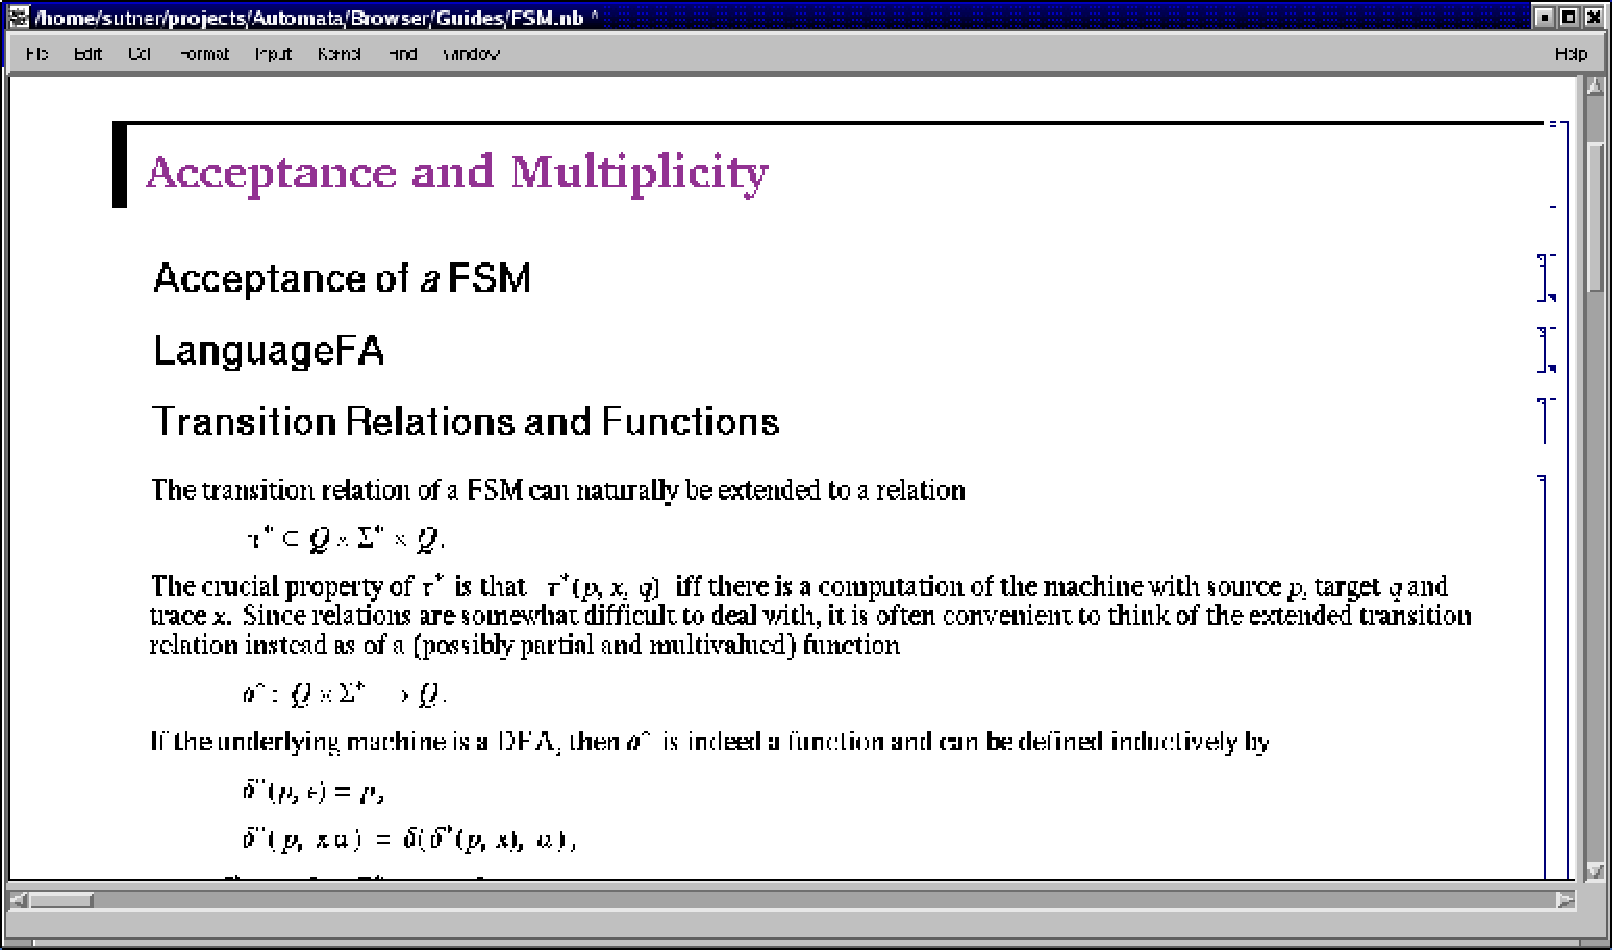
\includegraphics[width=10cm]{projects/mathematica/autosrc}
\end{myfig}

In order to facilitate the translation process it is advisable to front-load the
process: the author of the notebook is encouraged to use a special notebook
stylesheet, {\snippet{OMDocStyle.nb}}, that defines a number of syntactic categories
normally absent in a notebook.  These categories are implemented as a combination
of the cell types and cell labels.  As a typical example, consider a proof of some
assertion such as a theorem.  Ordinarily, a sequence of plain text cells would be
used to express a proof since none of the standard {\mathematica} stylesheets
provide a special proof style--though some have a theorem style.  The elements
defined in {\snippet{OMDocStyle.nb}} are easily accessible via pulldown menus or via
keyboard shortcuts in the notebook front end.  Moreover, the special styles are
color-coded in the notebook, so that it is easy for the author to see which
elements are present and which might be missing.


The conversion of mathematical expressions in the notebook is accomplished in a two-step
procedure.  First, we use the built-in {\mathematica} operation
{\snippet{ExpressionToSymbolicMathML}} that produces a symbolic expression representing a
MathML term that corresponds to the original notebook expression.  In a second,
post-processing step this expression is then transformed into an {\openmath} expression.
The post-processing relies heavily on the sophisticated pattern matching mechanism in
{\mathematica} and uses a special collection of rewrite rules.  The rules are based on
fairly simple-minded heuristics but do produce adequate results so long as the starting
expression is not too complicated.  As an example, consider the simple polynomial
expression $a x^2 + b x + c$ whose internal representation in {\mathematica} looks like so
(we assume here the expression appears inline within a block of text, the situation for an
input expression is entirely similar):
\begin{lstlisting}
Cell[ BoxData[FormBox[RowBox[{ 
      RowBox[{"a", " ", SuperscriptBox["x", "2"]}], "+", " ", 
      RowBox[{"b", " ", "x"}], " ", "+", " ", "c"}], 
        TraditionalForm]]]
\end{lstlisting}
The first conversion step produces the following {\mathematica} expression, 
shortened here to save space:
\begin{lstlisting}
XMLElement["math", 
  {"xmlns" ->"http://www.w3.org/1998/Math/MathML"}, 
  {XMLElement[ "apply", {}, {XMLElement["plus", {}, {}], 
   XMLElement[ "apply", {}, {XMLElement["times", {}, {}], 
     XMLElement["ci", {}, {"a"}], 
     XMLElement[ "apply", {}, {XMLElement["power", {}, {}], 
       XMLElement["ci", {}, {"x"}], 
       XMLElement["cn", {"type"->"integer"}, {"2"}]}]}], ...  }]}]
\end{lstlisting}
The post-processing finally yields the 
following expression, again shown only in part. 
\begin{lstlisting}
XMLElement["OMOBJ", {}, {XMLElement["OMA", {}, 
     {XMLElement["OMS", 
           {"cd"->"arith1", "name"->"plus"}, {}],
        XMLElement["OMA", {}, {XMLElement[ "OMS", 
           {"cd"->"arith1", "name"->"times"}, {}], 
        XMLElement["OMV", {"name"->"a"}, {}], 
        XMLElement["OMA", {}, {XMLElement["OMS", 
           {"cd"->"arith1", "name"->"power"}, {}], ...}]}]}]}]
\end{lstlisting}

The content dictionary was properly guessed in this instance.  Judging from the limited
experiments we have undertaken so far, it seems reasonable to expect that a fair amount of
the translation can be automated given that the field of discourse is limited, and that
the author is willing to customize the rewrite rules that control the post-processing
step.  Fortuitously, very little knowledge of {\mathematica} programming beyond some basic
syntax is necessary for the creation of these rules; mathematicians are likely to find
these rules fairly intuitive and natural.

At present, the conversion program is somewhat limited in its ability to deal with
arbitrarily structured notebooks.  It works well with a suite of notebooks developed
specifically for the {\snippet{OMDocStyle.nb}}, but requires modification for other types
of notebooks.  While it is not our goal to provide a truly general conversion tool with a
scope comparable to, say, the built-in conversion to MathML, some generalizations are
still needed at this point.

Another crucial issue is the extension of the rewrite rules used in the post-processing
step leading from MathML to {\openmath}.  No effort has been made so far to systematically
generate a set of rules suitable for a large class of documents.  At the very least, an
extension mechanism is needed that makes it easy for non-expert users to create the
necessary rule tables.

Lastly, it is desirable to create a {\mathematica} palette-based tool that focuses
more narrowly on the authoring and conversion of mathematical expressions only
rather than whole notebooks.  The generated raw {\openmath} expressions can be fed
directly into a low-level editor such as {\scsys{emacs}} using the special {\omdoc} mode
created as part of the {\ccaps} project, see elsewhere in this volume for a
description.

% LocalWords:  NotebookML evaluatable stylesheet OMDocStyle stylesheets BoxData
% LocalWords:  pulldown ExpressionToSymbolicMathML OpenMath FormBox RowBox nb
% LocalWords:  SuperscriptBox TraditionalForm XMLElement xmlns OMOBJ omdoc ci
% LocalWords:  arith CCaps thebib Sutner autosrc cn OMA cd OMV emacs

%%% Local Variables: 
%%% mode: latex
%%% TeX-master: "../../omdoc"
%%% End: 
